\PassOptionsToPackage{unicode}{hyperref}
\PassOptionsToPackage{hyphens}{url}

\documentclass[12pt,a4paper]{article}

\usepackage[T1]{fontenc}
\usepackage[utf8]{inputenc}
\usepackage[margin=1in]{geometry}
\usepackage{xcolor}
\usepackage{amsmath,amssymb,amsthm}
\usepackage{algorithm}
\usepackage{algpseudocode}
\usepackage{graphicx}
\usepackage{tikz}
\usepackage{float}
\usepackage{longtable,booktabs,array,tabularx}
\usepackage{calc}
\usepackage{etoolbox}
\IfFileExists{microtype.sty}{\usepackage{microtype}}{}
\usepackage{hyperref}
\usepackage{bookmark}
\IfFileExists{xurl.sty}{\usepackage{xurl}}{}
\urlstyle{same}
\usepackage{cite}

% ---------- theorem environments ----------
\theoremstyle{plain}
\newtheorem{theorem}{Theorem}[section]
\newtheorem{lemma}[theorem]{Lemma}
\newtheorem{proposition}[theorem]{Proposition}
\newtheorem{corollary}[theorem]{Corollary}
\theoremstyle{definition}
\newtheorem{definition}[theorem]{Definition}
\newtheorem{remark}[theorem]{Remark}

% ---------- math operators ----------
\DeclareMathOperator{\Runs}{Runs}
\DeclareMathOperator{\Inv}{Inv}
\DeclareMathOperator{\Rem}{Rem}
\DeclareMathOperator{\Exc}{Exc}
\DeclareMathOperator{\SortedSeq}{SortedSeq}
\newcommand{\tops}{\texttt{tops}}
\newcommand{\lastIdx}{\texttt{lastIdx}}

\makeatletter
\patchcmd\longtable{\par}{\if@noskipsec\mbox{}\fi\par}{}{}
\makeatother

\setcounter{secnumdepth}{3}
\setlength{\emergencystretch}{3em}

\hypersetup{
  pdftitle={LadderSort: Adaptive Sorting via Interleaved Nondecreasing Subsequences},
  hidelinks,
  pdfcreator={LaTeX}
}

\title{LadderSort: Adaptive Sorting via Interleaved\\Nondecreasing Subsequences}

\author{%
  Malik Mir Hamza Nayab\textsuperscript{1}%
  \thanks{Corresponding author. Email:
    \href{mailto:hamza.nayab48@gmail.com}{hamza.nayab48@gmail.com}}
  \and
  Ghanwa Batool\textsuperscript{2}%
  \thanks{Email:
    \href{mailto:ghanwa@cuiatd.edu.pk}{ghanwa@cuiatd.edu.pk}}\\[0.5em]
  \textsuperscript{1,2}COMSATS University Islamabad, Abbottabad Campus, Pakistan
}

\date{}

\begin{document}
\maketitle

% ============================================================
\begin{abstract}
Adaptive sorting algorithms exploit existing order in data to sort faster than $\Theta(N \log N)$, yet dominant methods such as TimSort measure presortedness by contiguous runs and degrade on inputs that are interleavings of sorted streams. We present LadderSort, a deterministic comparison-based sorting algorithm that adapts to $K$, the minimum number of nondecreasing subsequences covering the input, which equals both the offline optimum $K^*(A)$ and the length of the longest strictly decreasing subsequence $\mathrm{LDS}(A)$. The algorithm operates in two phases: Phase~1 decomposes the input into $K$ nondecreasing ladders via a hinted greedy scan, and Phase~2 merges them using a $K$-adaptive strategy (galloping two-way merge for $K=2$, loser-tree $K$-way merge for $K>2$). LadderSort runs in $O(N\log(K+1))$ time and $O(N+K)$ auxiliary space, interpolating between linear time on sorted input and $O(N\log N)$ on adversarial input. Experiments on eight synthetic workloads and a real GH~Archive trace ($K=368$) confirm practical speedups over TimSort on small-$K$ interleaved inputs while preserving graceful degradation on adversarial inputs.
\end{abstract}

\noindent\textbf{Keywords:} adaptive sorting; presortedness measures;
nondecreasing subsequences; multiway merge; loser tree; streaming data

\newpage

% ============================================================
\section{Introduction}
\label{sec:intro}
% ============================================================

Sorting is among the most fundamental primitives in algorithm design.
It underpins database query processing, search-index construction,
stream-join operators, analytics pipelines, and event-driven
architectures.  Classical comparison-based algorithms achieve
$\Theta(N\log N)$ worst-case time, which is information-theoretically
optimal for arbitrary inputs.  However, data encountered in practice is
rarely arbitrary.  In many modern systems the input to a sort routine
arrives not as a random permutation but as a {\em fan-in} of several
locally ordered producer streams, such as event logs from distributed services,
timestamped telemetry from a fleet of devices, social-media timelines
merged for display, posting-list segments in search-index maintenance,
venue-specific feeds in market-data processing, or partition outputs in
data-pipeline fan-in stages.  Each producer emits a nondecreasing stream,
and the aggregate sequence that reaches the sorting layer is a bursty,
noncontiguous interleaving of those streams.  Such sequences carry
substantial \emph{latent order} that a sufficiently adaptive algorithm
can exploit to sort well below the $N\log N$ barrier.

To understand why run-adaptive sorting is not enough, consider
the dominant family of adaptive sorting algorithms.  These algorithms, most notably
TimSort \cite{Auger2018} and PowerSort \cite{MunroWild2018}, measure
the exploitable order in a sequence $A$ by $\Runs(A)$, the number of
maximal contiguous monotone blocks (``runs'').  A contiguous run is only
useful when consecutive sorted elements appear next to each other in
memory.  In the fan-in workloads described above, each producer stream is
internally sorted, but records from different producers are interleaved
in the aggregate buffer.  The interleaving fragments each stream into
many short contiguous runs: every switch from one producer to another can
start a new run.  When context switches are frequent (the common case in
bursty telemetry, round-robin feed merging, or consolidated market
feeds), the run count satisfies $\Runs(A) = \Theta(N)$ even though the
sequence is an interleaving of only $K \ll N$ nondecreasing
subsequences.  Because the cost of run-adaptive algorithms is
$O(N + N\log\Runs(A))$, they are forced into $\Theta(N\log N)$
behavior on precisely the workloads that carry the most exploitable
structure.  A sorting algorithm that measures cost by the number of
interleaved sorted subsequences $K$ rather than by $\Runs(A)$ can sort
in $O(N\log(K+1))$ time, equivalently $O(N\log K)$ for $K \ge 2$, potentially orders of magnitude faster.

To illustrate the noncontiguous order problem, a simple example makes
the gap concrete.  Suppose three devices produce timestamped records:
\[
  D_1: 3,\;7,\;8 \qquad
  D_2: 2,\;5      \qquad
  D_3: 4.
\]
An arrival buffer that interleaves these streams might contain
$A = \langle 3,\;7,\;2,\;5,\;4,\;8 \rangle$.
A run-adaptive algorithm would see several short contiguous runs
($\langle 3,7 \rangle$, then a drop to~2, and so on), yielding a high
run count relative to $N$.  Yet the sequence is naturally explained as
three nondecreasing subsequences (ladders) that can be recovered
by a single left-to-right scan:
$L_1 = (3,7,8)$, $L_2 = (2,5)$, $L_3 = (4)$.
Once the ladders are identified, a 3-way merge produces sorted output.
LadderSort is built around exactly this observation: decompose the input
into a small number of nondecreasing ladders and then merge them
adaptively.

In our approach, LadderSort is a deterministic, comparison-based sorting
algorithm that operates in two phases.

\emph{Phase~1 (decomposition)} scans the input $A$ from left to right.
Each key $x$ is appended to the leftmost ladder whose current tail is at
most $x$; if no such ladder exists, a new ladder is created.  The
resulting decomposition produces $K$ nondecreasing ladders.
\emph{Phase~2 (adaptive merge)} merges the $K$ ladders using a strategy
selected by $K$: direct return for $K=1$, a galloping two-way merge for
$K=2$, and a loser-tree $K$-way merge for $K > 2$.  The combined cost is
$O(N\log(K+1))$ time, equivalently $O(N\log K)$ for $K \ge 2$, and $O(N+K)$ auxiliary space.

The parameter $K$ is not an arbitrary tuning knob.  Under the paper's
placement rule, the online ladder count $K_{\mathrm{LS}}(A)$ equals the
offline optimum $K^*(A)$ (the minimum number of nondecreasing
subsequences covering $A$), which in turn equals $\mathrm{LDS}(A)$, the
length of the longest strictly decreasing subsequence.  That is,
$K_{\mathrm{LS}}(A) = K^*(A) = \mathrm{LDS}(A)$; the formal proof
appears in Theorem~\ref{thm:greedy_optimal}.  LadderSort is therefore
strongest on inputs with small $K$ but many contiguous runs, exactly the
interleaved-stream workloads that defeat run-adaptive methods.

\subsection{Contributions}
This paper makes the following contributions.

\begin{enumerate}
  \item We present the full LadderSort algorithm:
    Phase~1 decomposes the input into nondecreasing ladders via a
    hinted placement search; Phase~2 merges them with a $K$-adaptive
    strategy.  The algorithm runs in $O(N\log(K+1))$ time and
    uses $O(N+K)$ auxiliary space.  Complete pseudocode is provided for
    all subroutines (Section~\ref{sec:algorithm}).

  \item We prove correctness (Lemmas~1--3, Theorem~1),
    establish that $K_{\mathrm{LS}}(A) = K^*(A) = \mathrm{LDS}(A)$
    (Theorem~\ref{thm:greedy_optimal}), derive time and space complexity
    bounds (Lemma~4), and provide an average-case analysis for uniform
    random permutations (Section~\ref{sec:theory}).

  \item We situate $K$ among the
    classical presortedness measures $\Runs$, $\Inv$, $\Rem$, and $\Exc$,
    showing that $K$ is complementary to $\Runs$: it captures
    noncontiguous order that $\Runs$ cannot distinguish from disorder
    (Section~\ref{sec:related}).

  \item We evaluate a hybrid variant that
    monitors $K$ during decomposition and falls back to a standard
    $O(N\log N)$ sort when $K$ exceeds a configurable threshold,
    protecting against adversarial high-$K$ inputs without penalizing
    the small-$K$ path (Section~\ref{sec:results}).

  \item A reproducible experimental suite
    covers eight synthetic workloads, a controlled $K$-sweep at
    $N = 10^7$, ablation experiments isolating each design choice,
    comparison-count and memory measurements, and a real GH~Archive event
    trace with measured $K = 368$, confirming LadderSort's practical
    benefits on small-$K$ interleaved-stream inputs while preserving
    graceful $\Theta(N\log N)$ behavior on adversarial workloads
    (Sections~\ref{sec:setup}--\ref{sec:results}).
\end{enumerate}


% ============================================================
\section{Related Work}
\label{sec:related}
% ============================================================

\subsection{Existing Presortedness Frameworks}
\label{sec:measures}

Adaptive sorting theory formalizes algorithmic cost as a function of a
\emph{measure of presortedness}, a function $m$ mapping sequences to
non-negative integers that satisfies monotonicity and normalization
axioms \cite{Mannila1985}.  Mannila's foundational framework establishes
that a measure $m$ is meaningful for adaptive sorting only if there exists an
algorithm whose comparison count is bounded by a function of $m(A)$ rather
than $N$ alone.  Crucially, the framework also shows that an algorithm
optimal with respect to measure $m_1$ need not be optimal with respect to
$m_2$ when the two measures are not mutually bounded; different measures
capture genuinely different kinds of order.

Estivill-Castro and Wood \cite{EstivillWood1992} survey the full hierarchy
of classical measures, including the number of contiguous runs $\Runs(A)$,
the inversion count $\Inv(A)$, the removal distance $\Rem(A)$, and the
exchange distance $\Exc(A)$ (each now formally defined in
Section~\ref{sec:prelim}, Definition~\ref{def:measures}).  These measures
are partially ordered by discriminating power: for example,
$\Inv(A) \ge \Runs(A) - 1$ for all $A$, so any algorithm optimal in $\Inv$
is at least as adaptive as one optimal in $\Runs$, but the converse does not
hold.

The measure $\SortedSeq(A)$ (the minimum number of nondecreasing
subsequences whose union covers $A$) occupies a distinctive position in
this hierarchy.  By Dilworth's Theorem \cite{Dilworth1950},
$\SortedSeq(A)$ equals the length of the longest strictly decreasing
subsequence $\mathrm{LDS}(A)$, connecting combinatorial covering to
extremal subsequence theory.
The $K$ parameter of LadderSort targets precisely this measure: we show
in Theorem~\ref{thm:greedy_optimal} that the online ladder count
$K_{\mathrm{LS}}(A)$ equals $\SortedSeq(A) = \mathrm{LDS}(A)$.

A large body of work exploits \emph{contiguous} monotone runs.
\emph{Natural mergesort} scans for such runs and merges them
\cite{Knuth1998}.  \emph{TimSort} \cite{Auger2018}, the most widely
deployed variant, detects ascending or descending runs, enforces minimum
run lengths via binary insertion sort, and controls merge order via
carefully chosen stack invariants; its complexity is $O(N + N\log\Runs(A))$.
\emph{PowerSort} \cite{MunroWild2018} improves merge scheduling to achieve
near-optimal merge trees with $O(N\log\Runs(A))$ comparisons and negligible
overhead; its multiway extension \cite{GellingNebel2023} further reduces
constants.  \emph{AdaptiveShiversSort} \cite{Juge2020} provides alternative
merge policies with entropy-style $NH + O(N)$ bounds on comparison counts.

Skiena's \emph{encroaching lists} \cite{Skiena1988} construct monotone
subsequences by greedily extending lists from either end (front or back),
yielding a presortedness measure that captures broader structure than
$\Runs$.  The number of encroaching lists lies between $\SortedSeq(A)$ and
$\Runs(A)$ in general.  Patience sorting \cite{AldousDiaconis1999} is a
classical online greedy procedure whose pile count corresponds to extremal
subsequence lengths (LIS or LDS, depending on tie convention).

General-purpose comparison sorts, such as Introsort \cite{BentleyMcIlroy1993,CLRS2022}
(the backbone of \texttt{std::sort}), BlockQuicksort \cite{Edelkamp2016},
and Smoothsort \cite{Dijkstra1981}, achieve $O(N\log N)$ worst case but
do not parameterize cost by any presortedness measure.

Tournament trees and their \emph{loser-tree} variant are classical
structures for $K$-way external-memory merging \cite{Knuth1998}.  A loser
tree of $K$ leaves initializes in $O(K)$ time and supports
extract-minimum-and-advance in $O(\log K)$ time, writing only
$\lceil \log K \rceil$ comparison results per step rather than
$2\lceil\log K\rceil$ as in a winner tree.  External-sort
contexts \cite{Aggarwal1988,Polyntsov2022} exploit this property when $K$
streams do not fit in memory.

\subsection{The Interleaving Gap}
\label{sec:interleaving_gap}

All of the run-adaptive methods surveyed above (TimSort, PowerSort,
AdaptiveShiversSort, and natural mergesort) measure cost as a function of
$\Runs(A)$, the number of \emph{contiguous} maximal monotone blocks.  This
measure is well suited to inputs that arrive as a few long sorted segments
(e.g., nearly sorted files, log rotations, append-dominated tables), but it
is structurally blind to \emph{noncontiguous} order.

Consider $K$ producer streams, each internally sorted, that are multiplexed
into a single buffer in arrival order.  Each producer contributes roughly
$N/K$ elements, and every context switch from one producer to another can
break a contiguous run.  When context switches are frequent (the common case
in bursty telemetry, round-robin feed merging, or consolidated market
feeds), the number of contiguous runs satisfies
$\Runs(A) = \Theta(N)$ even though the sequence is an interleaving of only
$K$ nondecreasing subsequences.  Because
$O(N + N\log\Runs(A)) = O(N\log N)$ when $\Runs(A)=\Theta(N)$, run-adaptive
sorts are forced into their worst-case behavior on precisely the workloads
that carry the most exploitable structure.

The core issue is a mismatch between the structural parameter and the
algorithmic measure.  The useful parameter is $K = \SortedSeq(A)$, the
minimum number of nondecreasing subsequences covering $A$.  For the
interleaved-stream scenario above, $K \ll N$ and often $K \ll \Runs(A)$;
an algorithm that adapts to $K$ rather than $\Runs(A)$ can sort in
$O(N\log(K+1))$ time, equivalently $O(N\log K)$ for $K \ge 2$, potentially orders of magnitude faster than
$O(N\log N)$.

Encroaching lists \cite{Skiena1988} partially address this gap by
capturing broader subsequence structure, but they function primarily as a
measure rather than a complete sorting algorithm: no deterministic merge
strategy with a proven $O(N\log(K+1))$ bound is specified.  Patience
sorting \cite{AldousDiaconis1999} achieves the optimal pile count but
likewise lacks an integrated $K$-adaptive merge phase.

To place the measure $K$ in context, LadderSort is parameterized by the ladder count produced by its online greedy
placement rule (Definition~\ref{def:placement}); we write
$K_{\mathrm{LS}}(A)$ for this quantity.  Theorem~\ref{thm:greedy_optimal}
proves that this online count equals the offline optimum $K^*(A)$, which in
turn equals $\mathrm{LDS}(A)$.  In particular
\[ K_{\mathrm{LS}}(A) = K^*(A) = \mathrm{LDS}(A) \le \Runs(A). \]
The rightmost inequality reflects that noncontiguous order, that is, order spread
across many short runs, can still be captured by a small number of ladders.
Concretely, if $A$ is an interleave of $K_0$ nondecreasing streams,
then $K_{\mathrm{LS}}(A) \le K_0$; equality holds when the interleaving contains a
strictly decreasing subsequence of length $K_0$.  In such cases, $\Runs(A)$ can be
$\Theta(N)$ while LadderSort achieves optimal decomposition.  Regarding inversions, one has
\(\Inv(A) \ge \binom{K}{2}\) for some natural orderings, so
\(K = O(\sqrt{\Inv(A)})\) in the worst case over sequences.

\subsection{Offline Sequence Decomposition: Dilworth's Theorem}
\label{sec:dilworth}

The minimum number of nondecreasing subsequences needed to cover $A$ is
governed by the \emph{longest strictly decreasing subsequence} of $A$, a
classical consequence of Dilworth's Theorem \cite{Dilworth1950} applied to
the partial order induced by the non-inversion relation.

\begin{proposition}[Dilworth equality for sequences]
\label{prop:dilworth}
For any sequence $A$, let $K^*(A) := \SortedSeq(A)$ be the minimum number
of nondecreasing subsequences that cover $A$, and let $\mathrm{LDS}(A)$ be
the length of a longest strictly decreasing subsequence of $A$.  Then
\[ K^*(A) = \mathrm{LDS}(A). \]
\end{proposition}

\begin{proof}
This is the standard specialization of Dilworth's theorem to the partial
order on indices where $i \preceq j$ iff $i<j$ and $a_i \le a_j$.  Chains
correspond to nondecreasing subsequences and antichains correspond to
strictly decreasing subsequences, yielding the equality.
\end{proof}

The offline minimum $K^*(A)$ can be computed in $O(N\log N)$ time using
standard patience-sorting routines \cite{Fredman1975,AldousDiaconis1999}.
The following theorem shows that the online greedy placement used in
Phase~1 achieves this offline optimum under our placement/tie convention.

\begin{theorem}[Optimality of the greedy ladder decomposition]
\label{thm:greedy_optimal}
For every input sequence $A$,
\[ K_{\mathrm{LS}}(A) = K^*(A) = \mathrm{LDS}(A). \]
\end{theorem}

\begin{proof}
We prove that the invariant holds: after processing any prefix of $A$, for every
$j \in \{1, \ldots, K\}$ there exists a strictly decreasing subsequence $D_j$ of length $j$
in the processed prefix such that $D_j$ ends at the current value $\tops[j]$.

\emph{Base case.} After processing the first element $a_1$, we have $K=1$ and
$\tops[1] = a_1$. The witness $D_1 = [a_1]$ is a decreasing subsequence of length 1 ending at $a_1$.

\emph{Inductive step.} Assume the invariant holds before processing element $x := a_t$ and
the current ladder count is $K$. Let $j = \pi(x; \tops)$ be the first feasible index.

\textit{Case 1: $j = K+1$ (new ladder created).}
Then $x < \tops[p]$ for all $p \in [1..K]$, in particular $x < \tops[K]$.
By the invariant, there exists a decreasing subsequence $D_K$ of length $K$ ending at $\tops[K]$.
Since $x$ is the current element being processed, it occurs after all elements of $D_K$ in the input.
Define $D_{K+1} := D_K \oplus [x]$ (append $x$ to $D_K$). Then $D_{K+1}$ is strictly decreasing
(since $\tops[K] > x$), has length $K+1$, and ends at $x = \tops[K+1]$.
The old witnesses $D_1, \ldots, D_K$ remain valid (they did not change).

\textit{Case 2: $j \le K$ (existing ladder updated).}
Update $\tops[j]$ to $x$. For all $p < j$, we have $\tops[p] > x$ (by definition of $j$ being first feasible).

If $j = 1$, set $D_1 := [x]$, a decreasing subsequence of length 1 ending at $x = \tops[1]$.

If $j > 1$, by the invariant there exists a decreasing subsequence $D_{j-1}$ of length $j-1$
ending at the old $\tops[j-1]$. Since $\tops[j-1] > x$ and $x$ occurs after all elements of
$D_{j-1}$ in the input, define $D_j := D_{j-1} \oplus [x]$. Then $D_j$ is strictly decreasing,
has length $j$, and ends at $x = \tops[j]$ (the new value).

For $q \in \{1, \ldots, j-1\}$: the values $\tops[q]$ do not change, so keep the witness $D_q$.

For $q \in \{j+1, \ldots, K\}$: the values $\tops[q]$ do not change, so keep the witness $D_q$.

Thus the invariant is maintained in all cases.

In conclusion, when Phase~1 terminates with $K$ ladders, the invariant guarantees
a strictly decreasing subsequence $D_K$ of length $K$ in the processed input $A$.
Therefore $\mathrm{LDS}(A) \ge K_{\mathrm{LS}}(A)$.

Conversely, LadderSort produces a valid cover of $A$ by $K_{\mathrm{LS}}(A)$ nondecreasing
subsequences (the ladders), so $K^*(A) \le K_{\mathrm{LS}}(A)$.
Also, any strictly decreasing subsequence of length $r$ requires $r$ distinct nondecreasing
subsequences in any cover, so $\mathrm{LDS}(A) \le K^*(A)$.
By Dilworth's Theorem (Proposition~\ref{prop:dilworth}), $K^*(A) = \mathrm{LDS}(A)$.

Combining these inequalities:
\[ \mathrm{LDS}(A) \ge K_{\mathrm{LS}}(A), \quad K^*(A) \le K_{\mathrm{LS}}(A), \quad K^*(A) = \mathrm{LDS}(A). \]
Therefore $K_{\mathrm{LS}}(A) = K^*(A) = \mathrm{LDS}(A)$.
\end{proof}

\subsection{LadderSort's Improvements}
\label{sec:improvements}

LadderSort closes the interleaving gap identified in
Section~\ref{sec:interleaving_gap} through three integrated design
decisions.

\subsubsection{Online chain decomposition with provable optimality}
Phase~1 decomposes the input into nondecreasing subsequences (ladders) using
a left-to-right online placement rule that assigns each element to the
leftmost feasible ladder (Definition~\ref{def:placement}).  The tail array
$\tops$ is maintained in strictly decreasing order
(Lemma~\ref{lem:tops_nonincreasing}), so the placement search reduces to
finding the leftmost position $j$ with $\tops[j] \le x$.  This is a
specialization of the patience-sorting family \cite{AldousDiaconis1999};
with our nonincreasing tail array and the ``$\le$'' placement predicate,
the greedy rule produces exactly $K^*(A) = \mathrm{LDS}(A)$ ladders
(Theorem~\ref{thm:greedy_optimal}).  Unlike prior work that treats the
decomposition as a stand-alone measure or an offline computation, LadderSort
uses it as the first stage of a complete sorting algorithm.

\subsubsection{Minimizing search overhead via hinting}
The placement search over the tail array is accelerated by a three-stage
hinted search (\textsc{HintedLowerBound}, Algorithm~\ref{alg:hinted}):
(i)~a local probe at the previous insertion index, exploiting temporal
locality when consecutive elements come from the same producer;
(ii)~an exponential gallop from the hint position;
(iii)~a binary search over the bounded interval.  This yields $O(\log K)$
worst-case cost per element, but in practice most elements are placed in
$O(1)$ time when the input exhibits producer-stream locality, precisely the
scenario where $K \ll \Runs(A)$.

\subsubsection{Deterministic multi-way merge}
Phase~2 selects a merge strategy by $K$: direct return for $K=1$, galloping
two-way merge (Algorithm~\ref{alg:gallop}) for $K=2$, and a loser-tree
$K$-way merge (Algorithm~\ref{alg:loser}) for $K > 2$.  The loser tree
performs one upward pass of $\lceil \log K \rceil$ comparisons per output
element.  Ties are broken deterministically by ladder identifier
(Definition~\ref{def:tiebreak}), ensuring reproducible output order.
The combined cost of decomposition and merge is
$O(N\log(K+1))$, equivalently $O(N\log K)$ for $K \ge 2$, with $O(N+K)$ auxiliary space.

\subsubsection{Hybrid guardrail}
For high-$K$ inputs (where $K$ approaches $N$ and LadderSort's overhead
exceeds that of a non-adaptive sort), a hybrid variant monitors $K$ during
decomposition and falls back to a standard $O(N\log N)$ sort when $K$
exceeds a configurable threshold.  This preserves LadderSort's small-$K$
path without penalizing adversarial inputs.

\section{Preliminaries and Notation}
 
Let $A = \langle a_1, a_2, \ldots, a_N \rangle$ be a sequence of $N$ keys drawn from a totally ordered domain $(\mathcal{D},\leq)$. We write $[m] := \{1,2,\ldots,m\}$. The goal is to compute a nondecreasing permutation $S$ of $A$. Throughout, ``sorted'' means nondecreasing under $\leq$. We use $\log$ to denote $\log_2$.
 
Table~\ref{tab:notation} summarizes the primary mathematical notations used throughout this paper.
 
\begin{table}[h]
\centering
\caption{Summary of mathematical notation.}
\label{tab:notation}
\begin{tabular}{ll}
\toprule
Notation & Description \\
\midrule
$A,N$ & Input sequence $A=\langle a_1,\ldots,a_N\rangle$ and its length $N$ \\
$K$ & Dynamic number of ladders (nondecreasing subsequences) produced by the algorithm \\
$K_{\mathrm{LS}}(A)$ & Formal function mapping $A$ to the ladder count produced by Phase~1 \\
$K^*(A)$ & Offline optimum: minimum number of nondecreasing subsequences covering $A$ \\
$\mathrm{LDS}(A)$ & Length of the longest strictly decreasing subsequence of $A$ \\
$\mathtt{tops}[1..K]$ & Contiguous array maintaining the tail (maximum) element of each active ladder \\
$\pi(x;\mathtt{tops})$ & Placement index: leftmost ladder $j$ such that $\mathtt{tops}[j] \leq x$ \\
$\oplus$ & Sequence concatenation operator (used in proofs) \\
$\prec$ & Total order for deterministic tie-breaking by ladder identifier during the merge \\
\bottomrule
\end{tabular}
\end{table}
 
\begin{definition}[Classical presortedness measures]
\label{def:measures}
\begin{align}
\mathrm{Runs}(A) &:= \text{number of maximal nondecreasing contiguous blocks in }A. \\
\mathrm{Inv}(A) &:= \bigl|\{(i,j) : i < j,\, a_i > a_j\}\bigr|. \\
\mathrm{Rem}(A) &:= N - \text{length of longest nondecreasing subsequence of }A. \\
\mathrm{Exc}(A) &:= \text{minimum number of exchanges/transpositions to sort }A. \\
\mathrm{SortedSeq}(A) &:= \text{minimum number of nondecreasing subsequences whose union covers }A.
\end{align}
\end{definition}
 
\begin{definition}[Ladder]
\label{def:ladder}
A \emph{ladder} is a finite sequence $L = \langle \ell_1, \ldots, \ell_m \rangle$ with $\ell_1 \leq \ell_2 \leq \cdots \leq \ell_m$.
\end{definition}
 
\begin{definition}[Tail and tail array]
\label{def:tail}
For a nonempty ladder $L$, its \emph{tail} is $\mathrm{tail}(L) := \ell_m$. During Phase~1 the algorithm maintains a sequence of ladders $(L_1,\ldots,L_K)$ and an auxiliary array $\mathtt{tops}[1..K]$ where $\mathtt{tops}[j] := \mathrm{tail}(L_j)$. The Phase~1 invariant is:
\[
  \mathtt{tops}[1] \geq \mathtt{tops}[2] \geq \cdots \geq \mathtt{tops}[K].
\]
\end{definition}
 
\begin{definition}[Placement index]
\label{def:placement}
For a key $x$ and a nonincreasing array $\mathtt{tops}[1..K]$, the \emph{placement index} is
\[
  \pi(x;\mathtt{tops}) := \min\bigl\{j \in [K] : \mathtt{tops}[j] \leq x\bigr\},
\]
taking $\pi(x;\mathtt{tops}) := K+1$ if no such $j$ exists.
\end{definition}
 
\begin{definition}[Algorithm-dependent ladder count $K$]
\label{def:K}
Let $(L_1,\ldots,L_K)$ be the ladders constructed by Phase~1 using the placement rule of Definition~\ref{def:placement}. We write $K_{\mathrm{LS}}(A) := K$ for the ladder count produced by LadderSort on input $A$; equivalently $K_{\mathrm{LS}}(A) = |\mathtt{tops}|$ at the end of Phase~1. When we refer to the offline optimum we write $K^*(A) := \mathrm{SortedSeq}(A)$.
\end{definition}
 
\begin{definition}[Run-identifier tie-break]
\label{def:tiebreak}
During $K$-way merge, comparisons use the total order:
\[
  (x,j) \prec (y,\ell) \iff (x < y) \vee (x = y \wedge j < \ell),
\]
where $j, \ell \in [K]$ are ladder identifiers assigned in creation order. This makes the merge deterministic on duplicate keys. Note that the algorithm is not globally stable.
\end{definition}
 
%-----------------------------------------------------------------------
% ============================================================
\section{The LadderSort Algorithm}
\label{sec:algorithm}
% ============================================================

\subsection{Overview}

LadderSort operates in two phases.
\textbf{Phase~1} (decomposition) scans $A$ left-to-right, assigning each key
to the leftmost feasible ladder (Definition~\ref{def:placement}) and
maintaining the tail array invariant.  \textbf{Phase~2} (adaptive merge)
merges the $K$ ladders using a strategy selected by $K$: direct return for
$K=1$, galloping two-way merge for $K=2$, and loser-tree $K$-way merge
for $K > 2$.

\begin{figure}[H]
\centering
\resizebox{\linewidth}{!}{%
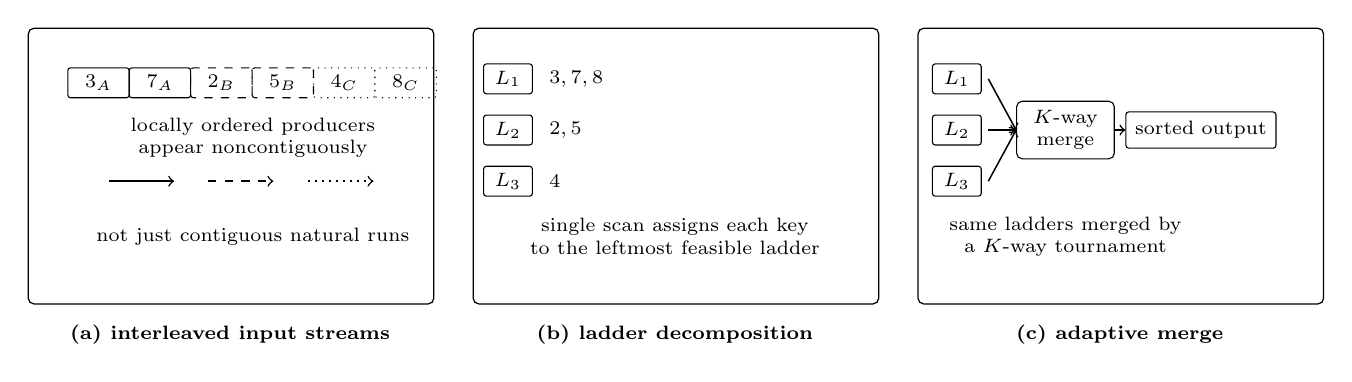
\begin{tikzpicture}[
  panel/.style={draw, rounded corners=2pt, line width=0.45pt,
    minimum width=5.15cm, minimum height=3.50cm, anchor=north west},
  token/.style={draw, rounded corners=1pt, minimum width=0.62cm,
    minimum height=0.38cm, inner sep=1pt, font=\scriptsize},
  stream/.style={draw, rounded corners=1pt, minimum width=0.78cm,
    minimum height=0.38cm, inner sep=1pt, font=\scriptsize},
  arrow/.style={->, line width=0.55pt},
  title/.style={font=\bfseries\scriptsize},
  note/.style={font=\scriptsize, align=center},
  every node/.style={font=\small}
 ]
\node[panel] (a) at (0,0) {};
\node[panel] (b) at (5.65,0) {};
\node[panel] (c) at (11.3,0) {};

\node[title] at (2.57,-3.90) {(a) interleaved input streams};
\node[title] at (8.22,-3.90) {(b) ladder decomposition};
\node[title] at (13.87,-3.90) {(c) adaptive merge};

\node[stream] at (0.90,-0.70) {\(3_A\)};
\node[stream] at (1.68,-0.70) {\(7_A\)};
\node[stream,dashed] at (2.46,-0.70) {\(2_B\)};
\node[stream,dashed] at (3.24,-0.70) {\(5_B\)};
\node[stream,dotted] at (4.02,-0.70) {\(4_C\)};
\node[stream,dotted] at (4.80,-0.70) {\(8_C\)};
\node[note] at (2.86,-1.40) {locally ordered producers\\appear noncontiguously};
\draw[arrow] (1.03,-1.95) -- (1.86,-1.95);
\draw[arrow,dashed] (2.29,-1.95) -- (3.12,-1.95);
\draw[arrow,dotted] (3.56,-1.95) -- (4.39,-1.95);
\node[note] at (2.86,-2.65) {not just contiguous natural runs};

\node[token] at (6.10,-0.65) {\(L_1\)};
\node[anchor=west, font=\scriptsize] at (6.50,-0.65) {\(3,7,8\)};
\node[token] at (6.10,-1.30) {\(L_2\)};
\node[anchor=west, font=\scriptsize] at (6.50,-1.30) {\(2,5\)};
\node[token] at (6.10,-1.95) {\(L_3\)};
\node[anchor=west, font=\scriptsize] at (6.50,-1.95) {\(4\)};
\node[note] at (8.22,-2.65) {single scan assigns each key\\to the leftmost feasible ladder};

\node[token] at (11.80,-0.65) {\(L_1\)};
\node[token] at (11.80,-1.30) {\(L_2\)};
\node[token] at (11.80,-1.95) {\(L_3\)};
\node[draw, rounded corners=2pt, minimum width=1.24cm, minimum height=0.64cm,
  font=\scriptsize, align=center] (merge) at (13.18,-1.30) {\(K\)-way\\merge};
\node[draw, rounded corners=1pt, minimum width=1.36cm, minimum height=0.46cm,
  font=\scriptsize] (out) at (14.90,-1.30) {sorted output};
\draw[arrow] (12.20,-0.65) -- (merge.west);
\draw[arrow] (12.20,-1.30) -- (merge.west);
\draw[arrow] (12.20,-1.95) -- (merge.west);
\draw[arrow] (merge.east) -- (out.west);
\node[note] at (13.18,-2.65) {same ladders merged by\\a $K$-way tournament};
\end{tikzpicture}%
}
\caption{LadderSort targets inputs that are interleavings of locally ordered
  streams.  Phase~1 decomposes the sequence into nondecreasing ladders by leftmost-feasible placement; in the example, $L_1=(3,7,8)$, $L_2=(2,5)$, and $L_3=(4)$.  Phase~2 merges them adaptively, yielding cost $O(N\log(K+1))$.}
\label{fig:overview}
\end{figure}

\subsection{Phase 1: Tail-Guided Decomposition}
\label{sec:phase1}

Algorithm~\ref{alg:laddersort} gives the full Phase~1 procedure.
The subroutine \textsc{HintedLowerBound} (Algorithm~\ref{alg:hinted})
implements $\pi(x;\tops)$ in $O(\log K)$ worst-case time using a
locality-aware three-stage search.



\subsubsection{Decomposition loop rationale}
The main decomposition loop processes the input in a single pass, tracking the active tail of each ladder in the \tops\ array. By caching and passing the most recently updated index (\lastIdx) into the search subroutine, the algorithm minimizes overhead for consecutive elements originating from the same locally ordered stream. This stateful tracking bridges the macroscopic fan-in structure of the input with the microscopic placement logic, ensuring that temporal locality is naturally exploited.

\begin{algorithm}[H]
\caption{\textsc{LadderSort}$(A)$}
\label{alg:laddersort}
\begin{algorithmic}[1]
\Require $A = \langle a_1, \dots, a_N \rangle$
\Ensure Sorted sequence $S$
\State Initialize empty ladder list $(L_1,\dots,L_K)$, $K \gets 0$
\State Initialize empty array $\tops$
\State $\lastIdx \gets 1$
\For{$i = 1$ to $N$}
    \State $x \gets a_i$
    \State $j \gets \textsc{HintedLowerBound}(\tops, x, \lastIdx)$
    \If{$j = K + 1$}
        \State $K \gets K + 1$;\quad $L_K \gets \langle x \rangle$;\quad $\tops[K] \gets x$
    \Else
        \State Append $x$ to $L_j$;\quad $\tops[j] \gets x$
    \EndIf
    \State $\lastIdx \gets j$
\EndFor
\State \Return $\textsc{MergeByK}(L_1, \dots, L_K)$
\end{algorithmic}
\end{algorithm}



\subsubsection{Hinted search rationale and layout of tops}
The three-stage search is designed to exploit the temporal locality of interleaved streams. Stage 1 (local probe) checks if the current element belongs to the same ladder as the immediately preceding element, providing an $O(1)$ placement for consecutive elements from the same producer. If the probe fails, Stage 2 (exponential gallop) bounds the search space before Stage 3 (binary search) finds the exact insertion point, guaranteeing an $O(\log K)$ worst-case bound while optimizing for the common case.

\begin{algorithm}[H]
\caption{\textsc{HintedLowerBound}$(\tops[1..K], x, \lastIdx)$}
\label{alg:hinted}
\begin{algorithmic}[1]
\Require Nonincreasing $\tops[1..K]$, key $x$, hint $\lastIdx$ valid when $K>0$
\Ensure First index $j \in [K]$ with $\tops[j] \le x$, or $K+1$
\If{$K = 0$}
    \State \Return $1$ \Comment{first element creates ladder 1}
\EndIf
\State \textbf{Stage 1 (local probe):} check $j = \lastIdx$
\If{$\tops[\lastIdx] \le x$}
    \State \Return $\lastIdx$ \Comment{same ladder as previous element}
\EndIf
\State \textbf{Stage 2 (exponential gallop):} starting from $\lastIdx$, double
  the stride $s \gets 1, 2, 4, \dots$ until $\tops[\lastIdx + s] \le x$ or $\lastIdx + s > K$
\State Let $[\mathit{lo}, \mathit{hi}]$ be the bounded search interval
\State \textbf{Stage 3 (binary search):} find the leftmost $j \in [\mathit{lo}, \mathit{hi}]$
  with $\tops[j] \le x$
\State \Return $j$ (or $K+1$ if none)
\end{algorithmic}
\end{algorithm}

The array $\tops[1..K]$ is allocated as a contiguous vector.  For small
values of $K$ the array is compact and is likely to reside in on-chip caches
on typical hardware, which makes the placement searches memory-friendly in
practice.  We avoid making precise hardware claims (cache sizes, branch
prediction behaviour, or TLB statistics) because such effects depend on the
target architecture and were not measured directly in our experiments.

\subsection{Phase 2: Adaptive Merge}
\label{sec:phase2}


\subsubsection{Adaptive merge rationale}
The merge control flow acts as a structural guardrail. For $K=1$, it bypasses merging entirely to achieve strict $O(N)$ linear time on already-sorted inputs. For $K=2$, it routes to a specialized two-way galloping merge to avoid the overhead of initializing a tournament tree. The $K$-way loser tree is strictly reserved for $K > 2$, ensuring that the heavier data-structure initialization and $\lceil \log K \rceil$ extraction costs are only paid when the fan-in complexity necessitates them
\begin{algorithm}[H]
\caption{\textsc{MergeByK}$(L_1, \dots, L_K)$}
\label{alg:mergebyk}
\begin{algorithmic}[1]
\Require Ladders $L_1, \dots, L_K$ (each nondecreasing)
\Ensure Globally sorted merge $S$
\If{$K = 0$} \Return $\langle\rangle$ \EndIf
\If{$K = 1$} \Return $L_1$ \EndIf
\If{$K = 2$} \Return $\textsc{TwoWayGalloping}(L_1, L_2)$ \EndIf
\State \Return $\textsc{KWayLoserTree}(L_1, \dots, L_K)$
\end{algorithmic}
\end{algorithm}



\subsubsection{Galloping merge rationale}
The galloping merge is utilized here specifically for the $K=2$ case to
exploit the long-range monotonic runs in the ladders, which allows skipping
over large segments of the input with $O(1)$ pointer increments, effectively
reducing comparison count on riffled interleavings \cite{Ghasemi2024}.  When two ladders
alternate in short bursts the gallop degrades gracefully to element-by-element
comparison; when one ladder dominates a long range the exponential search
identifies the entire block in $O(\log r)$ comparisons for a run of length
$r$, then advances the pointer in a single step.
\begin{algorithm}[H]
\caption{\textsc{TwoWayGalloping}$(L_1, L_2)$}
\label{alg:gallop}
\begin{algorithmic}[1]
\Require Sorted sequences $L_1$, $L_2$; pointers $p \gets 1$, $q \gets 1$
\Ensure Merged sorted sequence $S$
\While{$p \le |L_1|$ \textbf{and} $q \le |L_2|$}
    \State Compare heads $L_1[p]$ and $L_2[q]$
    \If{$L_1[p] \le L_2[q]$}
        \State \textbf{Gallop} in $L_1$: find the longest prefix $L_1[p..p+r-1] \le L_2[q]$ via exponential then binary search; emit it; $p \gets p + r$
    \Else
        \State \textbf{Gallop} in $L_2$: analogously find prefix $L_2[q..q+r-1] < L_1[p]$; emit; $q \gets q + r$
    \EndIf
\EndWhile
\State Emit remaining elements of whichever sequence is non-empty
\State \Return $S$
\end{algorithmic}
\end{algorithm}



\subsubsection{Loser-tree memory layout}
The loser tree is stored as an implicit binary tree in a flat array of $K$
integers (node indices), mirroring the heap-array layout \cite{Knuth1998}.
The winner pointer $T[0]$ and the $K-1$ internal loser nodes occupy
$K$ words; the $K$ head pointers occupy another $K$ words.  For moderate
values of $K$ the loser-tree state is compact and often fits in on-chip
caches.  The upward path from any leaf traverses $\lceil\log K\rceil$
nodes; these layout choices are intended to be efficient in practice
for typical memory hierarchies, but we avoid claiming specific cache-level or branch-prediction benefits
without empirical measurements on the target hardware.
\begin{algorithm}[H]
\caption{\textsc{KWayLoserTree}$(L_1, \dots, L_K)$}
\label{alg:loser}
\begin{algorithmic}[1]
\Require $K$ nondecreasing sequences; comparison order $\prec$ (Definition~\ref{def:tiebreak})
\Ensure Globally sorted merge $S$
\State Allocate internal loser-tree array $T[0..K-1]$ (node 0 = overall winner)
\State Initialize: for $j = 1$ to $K$, $\mathit{head}[j] \gets$ first element of $L_j$
\State Run $K-1$ comparisons to build initial tournament; record losers at each internal node
\While{any sequence non-empty}
    \State $j^* \gets T[0]$ \Comment{index of overall winner (minimum)}
    \State Emit $\mathit{head}[j^*]$
    \State Advance $L_{j^*}$ by one element; update $\mathit{head}[j^*]$ (or $+\infty$ if exhausted)
    \State Walk path from leaf $j^*$ to root, comparing with stored losers and updating $T$
    \Comment{$\lceil \log K \rceil$ comparisons; each node stores loser, so path = single upward pass}
\EndWhile
\State \Return $S$
\end{algorithmic}
\end{algorithm}

% ============================================================
\section{Theoretical Analysis}
\label{sec:theory}
% ============================================================

\subsection{Correctness}
\label{sec:correctness}

\begin{lemma}[Each ladder remains sorted]
\label{lem:ladder_sorted}
After processing any prefix $\langle a_1, \dots, a_t \rangle$ in Phase~1,
every ladder $L_j$ is nondecreasing.
\end{lemma}

\begin{proof}
Induction on $t$.  Base case $t=1$: $L_1 = \langle a_1 \rangle$ is
trivially nondecreasing.  Inductive step: assume all ladders are
nondecreasing after processing $a_1, \dots, a_{t-1}$.  At step $t$,
$x = a_t$ is assigned to ladder $L_j$ where $j = \pi(x;\tops)$.  If
$j = K+1$, a new singleton ladder $\langle x \rangle$ is created, which
is sorted.  Otherwise, $j$ is the first index with $\tops[j] \le x$, so
$\tops[j] = \mathrm{tail}(L_j) \le x$; appending $x$ to $L_j$ preserves
the nondecreasing property.  All other ladders are unchanged.
\end{proof}

\begin{lemma}[Strict tail invariant]
\label{lem:tops_nonincreasing}
After each insertion step of Phase~1 the tail array satisfies the strict
inequality
\[ \tops[1] > \tops[2] > \cdots > \tops[K]. \]
In particular the array is nonincreasing and, in fact, strictly decreasing
at all times.
\end{lemma}

\begin{proof}
We prove by induction on the number of processed elements that
$\tops[1] > \tops[2] > \cdots > \tops[K]$ is maintained.

\emph{Base case.} After the first insertion, $K=1$ and the invariant is vacuously true.

\emph{Inductive step.} Assume the invariant $\tops[1] > \tops[2] > \cdots > \tops[K]$ holds
before inserting element $x$. Let $j = \pi(x; \tops)$ be the first feasible index.

\textit{Case $j = K+1$ (new ladder).}
Then $x < \tops[p]$ for all $p \in [1..K]$, so $x < \tops[K]$.
We set $\tops[K+1] := x$. By the induction hypothesis, the old sequence
$\tops[1] > \cdots > \tops[K]$ is strictly decreasing. Since $x < \tops[K]$,
the new sequence $\tops[1] > \cdots > \tops[K] > \tops[K+1]$ is also strictly decreasing.

\textit{Case $j \le K$ (update existing ladder).}
We update $\tops[j] := x$.

For $p < j$: by definition of the first-feasible rule, $\tops[p] > x$. These values are unchanged.

For $p = j$: the new value is $x$.

For $p > j$: the values $\tops[p]$ are unchanged. By the induction hypothesis,
$\tops[j] > \tops[j+1]$ held before the update. Since the old $\tops[j] \le x$
(by feasibility), we have $\tops[j+1] < \tops[j] \le x$, thus $\tops[j+1] < x$.
After the update, the new value at position $j$ is $x$ and at position $j+1$ is $\tops[j+1]$,
so $x > \tops[j+1]$.

Boundary cases: If $j=1$, there are no positions $p<1$. If $j=K$, there are no positions $p>K$.
Both cases are covered by the logic above.

Therefore, the updated sequence $\tops[1] > \cdots > \tops[K]$ remains strictly decreasing.
\end{proof}

\begin{lemma}[Merge outputs a globally sorted list]
\label{lem:merge_sorted}
Assume $L_1, \dots, L_K$ are nondecreasing.  Then
$\textsc{MergeByK}(L_1, \dots, L_K)$ outputs a nondecreasing sequence $S$
that is a permutation of the multiset union $\bigcup_{j=1}^K L_j$.
\end{lemma}

\begin{proof}
\emph{$K \in \{0,1\}$:} Trivial.

\emph{$K = 2$:} \textsc{TwoWayGalloping} is a standard merge
(accelerated by galloping, which only extends contiguous blocks that are
provably $\le$ the opposing head).  Galloping does not alter correctness,
only the number of comparisons.  The result is a sorted permutation of
$L_1 \cup L_2$.

\emph{$K > 2$:} \textsc{KWayLoserTree} maintains one current head per
ladder and repeatedly outputs the minimum head under $\prec$
(Definition~\ref{def:tiebreak}).  Since each $L_j$ is nondecreasing,
advancing any pointer never decreases that ladder's head.  At each step,
the loser tree correctly identifies the global minimum head (by the
standard correctness argument for tournament trees \cite{Knuth1998}),
outputs it, advances the corresponding ladder, and restores the
tournament in $O(\log K)$ time.  Because $\prec$ is a total order
refining $\le$, the output sequence is nondecreasing in key order.
Every element is output exactly once, so $S$ is a permutation of the
union.
\end{proof}

\begin{theorem}[Correctness of LadderSort]
\label{thm:correctness}
For any input $A = \langle a_1, \dots, a_N \rangle$ over a totally
ordered domain, \textsc{LadderSort}$(A)$ outputs a sequence $S$ that is
(i) a permutation of $A$ and (ii) nondecreasing under $\le$.
\end{theorem}

\begin{proof}
By Lemma~\ref{lem:ladder_sorted}, each $L_j$ produced in Phase~1 is
nondecreasing.  Every element $a_i$ is appended to exactly one ladder
(or starts a new one), so the multiset union of the ladders equals $A$.
Lemma~\ref{lem:tops_nonincreasing} ensures the tail-array invariant is
maintained throughout, guaranteeing that the placement predicate is
applied correctly.  By Lemma~\ref{lem:merge_sorted}, Phase~2 outputs a
nondecreasing permutation of the union, which equals a nondecreasing
permutation of~$A$.
\end{proof}

\begin{figure}[H]
\centering
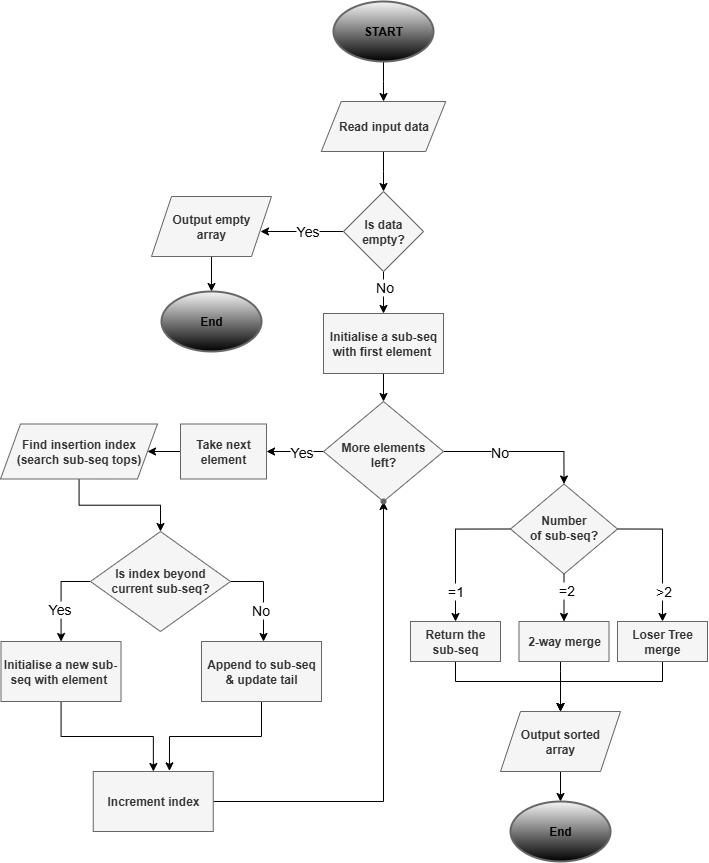
\includegraphics[width=0.82\linewidth]{media/image2.jpg}
\caption{Implementation flowchart of LadderSort. The diagram summarises the
  decomposition and merge control flow, complementing the conceptual
  overview in Figure~\ref{fig:overview}.}
\label{fig:laddersort-flowchart}
\end{figure}

\subsection{Time Complexity}
\label{sec:timecomplexity}

\begin{lemma}[Time complexity]
\label{lem:complexity}
\textsc{LadderSort} runs in $O(N\log(K+1))$ time. More precisely, the algorithm is linear for $K=1$ and runs in $O(N\log K)$ for $K \ge 2$.
\end{lemma}

\begin{proof}
\emph{Phase~1.}  Each of the $N$ elements requires one call to
\textsc{HintedLowerBound}.  Stage~1 (local probe) costs $O(1)$.
Stage~2 (exponential gallop) doubles the stride until it reaches a
feasible index or overshoots $K$; the number of doublings is
$O(\log K)$.  Stage~3 (binary search within the bounded interval of
length at most $2s \le 2K$) costs $O(\log K)$.  Hence each placement
costs $O(\log K)$ in the worst case, giving Phase~1 cost $O(N \log(K+1))$.

\emph{Phase~2.}  For $K = 1$, the merge is $O(N)$ (return the single ladder).
For $K = 2$, the merge is $O(N)$ (binary merge overhead).  For $K > 2$, \textsc{KWayLoserTree} builds in $O(K)$ time
and performs $N$ extract-minimum steps each costing $O(\log K)$, for
total $O(K + N\log K) = O(N\log K)$ (since $K \le N$).

Combining both phases: $T(N, K) = O(N\log(K+1))$.
\end{proof}

\begin{remark}
The bound $T(N,K)=O(N\log(K+1))$ interpolates correctly: $T(N,1)=O(N)$ and $T(N,N)=O(N\log N)$.  For $K = N^{o(1)}$ (e.g.\ $K = O((\log N)^c)$),
the cost is $o(N \log N)$.
\end{remark}


\subsection{Average-Case Analysis}
\label{sec:avgcase}

For a \emph{uniformly random permutation} of $N$ distinct keys, we bound the
expected value of $K$ produced by the LadderSort placement rule.

\begin{proposition}[Expected $K$ under uniform random permutation]
\label{prop:avgcase}
Let $A$ be a uniformly random permutation of $\{1, \dots, N\}$.  The
expected number of ladders produced by \textsc{LadderSort} satisfies
\[
  \mathbb{E}[K] = \Theta(\sqrt{N}).
\]
\end{proposition}

\begin{proof}
By Theorem~\ref{thm:greedy_optimal} we have $K=K_{\mathrm{LS}}(A)=\mathrm{LDS}(A)$.
Classical results on longest increasing/decreasing subsequences in random
permutations (Vershik--Kerov \cite{VershikKerov1977},
Logan--Shepp \cite{LoganShepp1977}, and the survey by
Aldous--Diaconis \cite{AldousDiaconis1999}) imply that the expected length
of the longest decreasing subsequence of a uniform random permutation of
$[N]$ is $\Theta(\sqrt{N})$ (in fact $2\sqrt{N}+o(\sqrt{N})$).  Hence
$\mathbb{E}[K]=\Theta(\sqrt{N})$.
\end{proof}

\begin{corollary}[Average-case complexity]
\label{cor:avgcase}
For a uniformly random permutation of $N$ distinct keys, classical results
on longest decreasing subsequences imply $\mathbb{E}[K]=\Theta(\sqrt{N})$.
Therefore, under the equality $K=\mathrm{LDS}(A)$ established above,
\[ \mathbb{E}[T(N,K)] = O\bigl(N\mathbb{E}[\log K]\bigr) = O(N\log\sqrt{N}) = O\bigl(N\tfrac{1}{2}\log N\bigr).
\]
The constant $\tfrac{1}{2}$ arises from the $\sqrt{N}$ scaling of $K$; one
may obtain the sharper $2\sqrt{N}+o(\sqrt{N})$ asymptotic for $\mathbb{E}[K]$
from Vershik--Kerov and Logan--Shepp via Aldous--Diaconis \cite{VershikKerov1977,LoganShepp1977,AldousDiaconis1999}.
\end{corollary}


This asymptotic is consistent with the empirical comparison counts in
Section~\ref{sec:results}: on random inputs LadderSort behaves like an
algorithm whose logarithmic factor is about $\tfrac{1}{2}\log N$ on average.

\subsection{A lower bound for the $K$-interleaving promise}
\label{sec:lowerbound}

To contextualise LadderSort's $O(N\log(K+1))$ bound, we give a simple
information-theoretic lower bound for the class of inputs that are
interleavings of $K$ labeled sorted subsequences.

\begin{proposition}[Worst-case comparison lower bound under $K$-interleaving]
\label{prop:lowerbound}
Consider the set of sequences formed by interleaving $K$ labeled sorted
subsequences whose total length is $N$ and whose lengths are balanced
(each about $N/K$).  Any comparison-based algorithm that correctly
distinguishes all such interleavings must perform at least
\(\Omega(N\log K)\) comparisons in the worst case.
\end{proposition}

\begin{proof}[Sketch]
The number of distinct interleavings of $K$ labeled subsequences of sizes
$n_1,\dots,n_K$ is the multinomial coefficient
\(\frac{N!}{n_1!\cdots n_K!}\).  For balanced lengths $n_j\approx N/K$ the
logarithm of this quantity is $\Theta(N\log K)$ by Stirling's formula, so
any decision tree distinguishing these inputs must have depth
\(\Omega(N\log K)\), implying the stated lower bound on comparisons.
\end{proof}

This lower bound is conditional on the promise that the input is an
interleaving of $K$ labeled sorted streams (so the algorithm need only
distinguish permutations consistent with that promise).  It does not
supersede the general $\Omega(N\log N)$ lower bound for arbitrary inputs;
rather, it shows that LadderSort's $O(N\log(K+1))$ behaviour is asymptotically
optimal (up to constant factors) for the restricted $K$-interleaving input
class when the streams are balanced.

\subsection{Space Complexity}
\label{sec:space}

\begin{lemma}[Space complexity]
\label{lem:space}
\textsc{LadderSort} uses $O(N + K)$ auxiliary space.
\end{lemma}

\begin{proof}
\emph{Phase~1 storage.}  Each element $a_i$ is stored in exactly one
ladder; the total storage for all ladder elements is $N$ words.  The
$\tops$ array uses $K$ additional words.  Hence Phase~1 auxiliary space
is $O(N + K) = O(N)$ (since $K \le N$).

\emph{Phase~2 storage.}  For $K \le 2$, a two-pointer merge uses $O(1)$
extra space beyond the output buffer.  For $K > 2$, the loser tree
stores $K$ internal nodes and $K$ head pointers, using $O(K)$ extra words
beyond the ladders.  The output array uses $N$ words.

\emph{Total.}  $O(N + K) = O(N)$ auxiliary words.
\end{proof}

\subsubsection{Comparison with merge-based sorts}
Standard top-down mergesort uses $O(N)$ auxiliary space (a scratch buffer).
\texttt{std::stable\_sort} on most implementations uses $O(N)$ space and
falls back to $O(N \log N)$-compare in-place variants when allocation fails.
LadderSort's space bound is comparable to these standard algorithms.
In the worst case ($K = N$, descending input), the ladder storage itself
is $O(N)$ singletons, but the total space is still $O(N)$.

\subsection{Implementation locality discussion}
\label{sec:io}

We discuss implementation-level locality considerations without asserting
tight cache-oblivious optimality.  Phase~1 scans the input sequentially and
maintains a compact contiguous tail array $\tops[1..K]$; for small $K$ this
structure is compact and tends to be efficient in practice.  Phase~2
performs $K$-way merges using per-ladder read buffers and a loser-tree over
the active heads; when the number of ladders and buffers fit in available
memory, multiway merging reduces the number of passes over the data versus
naive repeated two-way merging.  Exact I/O bounds and cache-oblivious
optimality depend on buffer management choices and hardware parameters $M$
and $B$, which we did not model or measure precisely in our experiments.
Hence we present empirical locality observations in Section~\ref{sec:results}
rather than formal cache-level theorems.

% ============================================================
\section{Experimental Setup}
\label{sec:setup}
% ============================================================

\subsection{Hardware and Compiler}

All experiments ran on a 2020 MacBook Air with an Apple M1 8-core CPU and
8\,GB unified memory under macOS 15.6.1.  Binaries were compiled with
Homebrew GCC~15 using:
\[
  \texttt{g++-15\ -O3\ -march=native\ -flto\ -funroll-loops\ -std=c++20}.
\]
All runs were single-threaded with no explicit SIMD.

\subsection{Algorithms}

\begin{itemize}
  \item \textbf{LadderSort} (raw): two-phase decomposition + adaptive merge.
  \item \textbf{Hybrid LadderSort}: monitors $K$ mid-decomposition; falls back
    when $K$ exceeds a threshold.
  \item \textbf{TimSort}: stable adaptive mergesort (\texttt{gfx::timsort}).
  \item \textbf{QuickSort}: three-way partitioning, median-of-three/ninther.
  \item \textbf{IntroSort}: \texttt{std::sort} (libstdc++).
  \item \textbf{StableSort}: \texttt{std::stable\_sort}.
  \item \textbf{MergeSort}: top-down stable mergesort with reusable buffer.
\end{itemize}

\subsection{Workloads and Measured $K$}
\label{sec:workloads}

Eight synthetic workloads span the structural range from $K=1$ to $K=N$.
Table~\ref{tab:measured-k} reports mean measured $K$ over 10 runs per size.
The controlled $K$-sweep fixes $N=10^7$ and varies target $K$ using
randomized exact-$K$ interleavings, with 10 timed rounds per configuration
after one warm-up.  Six of 400 rows (1.5\%) were filtered for system-level
paging outliers (time $> 10$\,s); all correctness checks passed.

\begin{table}[H]
\centering
\small
\caption{Mean measured ladder count $K$ over 10 runs. The suite spans
  $K=1$ (single sorted run) to $K=N$ (adversarial descending), covering the
  full structural range of LadderSort's parameterization.}
\label{tab:measured-k}
\begin{tabularx}{\linewidth}{@{}lrrrX@{}}
\toprule
Workload & $N=10^6$ & $N=10^7$ & $N=10^8$ & Interpretation \\
\midrule
Ascending       & 1.0    & 1.0    & 1.0     & Single ladder \\
Two-run riffle  & 2.0    & 2.0    & 2.0     & Two interleaved streams \\
Block-cyclic    & 8.0    & 8.0    & 8.0     & Eight producers \\
Band-limited    & 14.9   & 15.9   & 16.6    & Bounded local jitter ($W=32$) \\
Partial index   & 16.0   & 16.0   & 16.0    & Small segment fan-in \\
Social-feed     & 24.0   & 24.0   & 24.0    & Multi-source fan-in \\
Random          & 1985.8 & 6302.1 & 19955.1 & Weak structure \\
Descending      & $10^6$ & $10^7$ & $10^8$  & Worst case \\
\bottomrule
\end{tabularx}
\end{table}

% ============================================================
\section{Results and Discussion}
\label{sec:results}
% ============================================================

We report mean wall-clock time $\pm$ standard deviation over 10 runs
(median for the $K$-sweep).  Correctness is verified after every run.

\subsection{Controlled $K$-Sensitivity Sweep}

Figure~\ref{fig:k-sweep-runtime} shows median runtime vs.\ $K$ at $N=10^7$.
LadderSort's runtime rises monotonically with $K$, consistent with the
$O(N\log(K+1))$ bound, and with $O(N\log K)$ behavior for $K \ge 2$.  TimSort is fastest at $K=1$ (single already-sorted run);
LadderSort and Hybrid LadderSort lead for $2 \le K \lesssim 64$, where the
loser-tree merge exploits the small fan-in structure.

\begin{figure}[H]
\centering

\includegraphics[width=0.82\linewidth]{media/k_sweep_runtime_vs_k.pdf}
\caption{Controlled $K$-sweep at $N=10^7$.  Median runtime increases with
  $K$, consistent with the $O(N\log(K+1))$ bound, and with $O(N\log K)$ behavior for $K \ge 2$.  TimSort leads at $K=1$; LadderSort
  leads for small $K \ge 2$.}
\label{fig:k-sweep-runtime}
\end{figure}

\subsubsection{Implementation locality}
For small $K$, the $\tops$ array is compact (e.g., $K \le 64$ entries $= 256$\,bytes),
which may improve data locality in practice. Similarly, the loser tree layout uses
heap-array indexing to improve locality. As $K$ grows, the array size and tree depth increase,
which could affect cache behavior. The gradual runtime increase visible in
Figure~\ref{fig:k-sweep-runtime} is consistent with this trend, but we did not directly
measure cache misses or other hardware counters to confirm the mechanism.

\begin{figure}[H]
\centering

\includegraphics[width=0.82\linewidth]{media/k_sweep_speedup_vs_k.pdf}
\caption{Speedup vs.\ TimSort on the $K$-sweep.  LadderSort and Hybrid
  lead in the small-$K$ interleaved regime; advantage narrows as $K$ grows.}
\label{fig:k-sweep-speedup}
\end{figure}

\subsection{Workload-by-Workload Analysis}

\subsubsection{Uniform random ($K \approx \sqrt{N}$)}
On random input, \texttt{std::sort} (IntroSort) is fastest due to its
highly tuned in-place partitioning with minimal memory traffic and strong
branch prediction on pivot comparisons.  LadderSort is competitive but not
leading: Phase~1 placement incurs $O(\log K)$ cost per element with
$K \approx \sqrt{N}$, and Phase~2 runs a full $K$-way merge.  The measured
comparison counts ($\approx 21$ per element at $N=10^6$) match the
theoretical expectation of $\frac{1}{2}\log_2 N \approx 10$ for Phase~1
plus $\frac{1}{2}\log_2 N$ for Phase~2, summing to $\approx \log_2 N = 20$.

\begin{table}[H]
\centering\small
\caption{Runtime (s) on uniform random input: mean $\pm$ std.\ dev.\ over 10 runs.}
\begin{tabularx}{\linewidth}{@{}lrrrX@{}}
\toprule
Algorithm & $10^6$ & $10^7$ & $10^8$ & Note \\
\midrule
LadderSort     & 0.0603\,($\pm$0.0003) & 0.7115\,($\pm$0.0080) & 8.352\,($\pm$0.078) & Competitive \\
TimSort        & 0.0761\,($\pm$0.0006) & 0.8628\,($\pm$0.0007) & 10.021\,($\pm$0.065) & \\
QuickSort      & 0.0678\,($\pm$0.0002) & 0.7990\,($\pm$0.0006) & 9.367\,($\pm$0.133) & \\
IntroSort      & 0.0539\,($\pm$0.0005) & 0.6242\,($\pm$0.0009) & 7.286\,($\pm$0.079) & Fastest \\
StableSort     & 0.0612\,($\pm$0.0001) & 0.7128\,($\pm$0.0005) & 8.398\,($\pm$0.012) & \\
MergeSort      & 0.0680\,($\pm$0.0001) & 0.7756\,($\pm$0.0017) & 9.245\,($\pm$0.059) & \\
\bottomrule
\end{tabularx}
\end{table}

\subsubsection{Sorted ascending ($K=1$)}
LadderSort is linear ($K=1$: Phase~1 makes one ladder, Phase~2 returns it),
but pays bookkeeping overhead for the initial probe and array allocation.
TimSort is $10\times$ faster due to its optimized run-detection path that
avoids all comparisons beyond confirming the single ascending run and copies
the input directly.  This performance gap is not a flaw in LadderSort but
reflects that $K=1$ is TimSort's absolute best case.

\subsubsection{Sorted descending ($K=N$)}
This is LadderSort's worst case: every element starts a new ladder,
Phase~1 creates $N$ singletons, and Phase~2 runs an $N$-way merge consuming
$O(N)$ memory for the loser tree.  The 3.73\,GiB peak RSS at $N=10^8$
(Table~\ref{tab:phase5-memory}) reflects the $N$ singleton ladder pointers
and the $N$-node loser tree.  TimSort, by contrast, detects the descending
run in one pass and reverses it in $O(N)$ time and $O(1)$ extra space.
LadderSort's placement loop must create a new ladder for each element,
which may introduce different branch-prediction patterns than TimSort's
reversal loop, but we did not measure branch-misprediction rates directly.

\subsubsection{Band-limited nearly sorted ($K \approx 16$)}
LadderSort benefits from the small effective $K$: Phase~1 places each element
in $O(\log 16) = O(4)$ comparisons on average, and Phase~2 runs a 16-way
merge with a compact loser-tree structure.  The compact array and tree layouts
may improve data locality compared to larger $K$ values.  The effective time per element on
this workload is closer to the $K = 16$ regime than the average-case $\sqrt{N}$ regime.  StableSort is close,
reflecting that $K=16$ is moderate enough that a standard merge-sort tree also
benefits from the bounded jitter.

\subsubsection{Block-cyclic interleave ($K=8, B=4$)}
LadderSort leads across all sizes.  The block-cyclic pattern (8 sorted
producers emitting blocks of 4) means Phase~1 frequently encounters the same
ladder as the previous element, reducing placement overhead.  Phase~2 runs an
8-way merge with a compact loser tree (8 internal nodes + 8 head pointers).
The measured speedup over TimSort at $N=10^8$ is approximately $1.14\times$,
consistent with TimSort observing many short runs (of length $B=4$) and
incurring merge-scheduling overhead.

\subsubsection{Two-run riffle ($K=2$)}
After Phase~1 identifies the two ladders, Phase~2 reduces to a single
two-way galloping merge.  Galloping is particularly effective here: each
ladder contains $N/2$ elements arranged as a long sorted sequence, so
each gallop step skips $\Omega(\log N)$ elements before switching sides,
reducing total comparisons to $O(N)$ with a small constant.  LadderSort's
advantage over TimSort ($\approx 1.35\times$ at $N=10^8$) reflects TimSort's
overhead from observing $N/2$ short alternating runs and applying its
merge-scheduling stack logic.

\subsubsection{Social-feed fan-in ($K=24$) and partial-index merges ($K=16$)}
Both workloads produce small fixed $K$ with heavy duplicate keys.
LadderSort's deterministic tie-breaking (Definition~\ref{def:tiebreak})
ensures reproducible output on these tie-heavy inputs, which is important for
feed-construction and index-maintenance pipelines that require stable ordering
within timestamps.  Partition-based methods (\texttt{std::sort}) degrade on
equality plateaus due to poor three-way partitioning behavior when nearly all
elements are equal.

\subsection{Ablation Study}
\label{sec:ablation}

Table~\ref{tab:phase4-ablation} reports median relative runtime, normalized
to LadderFull $= 1.00$.  \emph{NoHint} disables Stage~1 of
\textsc{HintedLowerBound}; \emph{NoGallop} uses plain two-pointer merge for
$K=2$; \emph{HeapMerge} replaces the loser tree with a binary heap;
\emph{StableMode} enforces global stability via per-element input-position tracking.

\begin{table}[H]
\centering\small
\caption{Ablation results normalized to LadderFull $= 1.00$.  Values $> 1$
  are slower.  Hints and loser-tree merging matter most in the $K > 2$
  social-feed regime; galloping and hints show mixed results for $K=2$.}
\label{tab:phase4-ablation}
\begin{tabularx}{\linewidth}{@{}lXrrrrrr@{}}
\toprule
& & \multicolumn{3}{c}{Social-feed ($K=24$)} & \multicolumn{3}{c}{Two-run riffle ($K=2$)} \\
\cmidrule(lr){3-5}\cmidrule(lr){6-8}
Variant & Purpose & $10^6$ & $10^7$ & $10^8$ & $10^6$ & $10^7$ & $10^8$ \\
\midrule
LadderFull & Full implementation      & 1.00 & 1.00 & 1.00 & 1.00 & 1.00 & 1.00 \\
NoHint     & Disable hinted placement & 1.71 & 1.75 & 1.28 & 0.86 & 0.84 & 0.68 \\
NoGallop   & Disable galloping merge  & 0.97 & 0.99 & 0.72 & 1.07 & 1.06 & 0.79 \\
HeapMerge  & Heap instead of loser tree & 1.94 & 2.05 & 1.51 & 1.02 & 1.00 & 0.82 \\
StableMode & Enforce global stability  & 1.03 & 1.07 & 1.26 & 1.05 & 1.07 & 1.43 \\
\bottomrule
\end{tabularx}
\end{table}

\subsubsection{Implementation considerations for ablation}
The $1.51\times$--$2.05\times$ slowdown from \emph{HeapMerge} is explained by
the binary heap's two-child comparison per extract step versus the loser
tree's single upward-path pass: a heap on $K=24$ nodes requires
$2\lfloor\log_2 24\rfloor = 8$ comparisons per extract, while the loser tree
requires $\lceil\log_2 24\rceil = 5$ comparisons and a fixed search path (unlike
heap sifting, which has data-dependent branching). The \emph{NoHint} slowdown at $K=24$ ($1.28\times$
at $N=10^8$) reflects increased search overhead: without the local probe, Stage~2
begins exponential galloping from index~1 every time, which may increase memory
access costs. The \emph{StableMode} overhead at $N=10^8$
($1.26\times$ for social-feed, $1.43\times$ for two-run riffle) arises from
the additional $\log N$ bits per element needed to track original input positions
for tie-breaking.

\subsection{Hybrid LadderSort}
\label{sec:hybrid}

\begin{table}[H]
\centering\scriptsize
\caption{Hybrid LadderSort: fallback rate, speedup over Raw, and speedup over
  TimSort.  Hybrid falls back on high-$K$ inputs, preserving small-$K$ path.}
\label{tab:phase4-hybrid}
\begin{tabularx}{\linewidth}{@{}lrrrrrX@{}}
\toprule
Dataset & $N$ & Fallback & vs.\ Raw & vs.\ TimSort & Interpretation \\
\midrule
Descending   & $10^6$ & 1.00 & 5.71 & 0.07 & Avoids worst case \\
Descending   & $10^7$ & 1.00 & 6.36 & 0.07 & Avoids worst case \\
Descending   & $10^8$ & 1.00 & 4.14 & 0.03 & Avoids worst case \\
Random       & $10^6$ & 1.00 & 1.62 & 2.51 & Fallback improves over raw \\
Random       & $10^7$ & 1.00 & 1.67 & 2.66 & Fallback improves over raw \\
Random       & $10^8$ & 1.00 & 1.75 & 2.77 & Fallback improves over raw \\
Block-cyclic & $10^6$ & 0.00 & 0.90 & 1.81 & Preserves small-$K$ path \\
Block-cyclic & $10^7$ & 0.00 & 1.03 & 1.75 & Preserves small-$K$ path \\
Block-cyclic & $10^8$ & 0.00 & 1.12 & 1.66 & Preserves small-$K$ path \\
\bottomrule
\end{tabularx}
\end{table}

\subsection{Memory and Comparison Overheads}
\label{sec:overhead}

\begin{table}[H]
\centering\small
\caption{Peak resident set size at $N=10^8$ (GiB). Raw LadderSort's
  descending footprint of 3.73\,GiB reflects $K=N$ ladder storage; Hybrid
  avoids this by falling back.}
\label{tab:phase5-memory}
\begin{tabularx}{\linewidth}{@{}lrrrrX@{}}
\toprule
Dataset & Raw LS & Hybrid LS & TimSort & \texttt{std::sort} & \texttt{std::stable\_sort} \\
\midrule
Descending  & 3.73 & 1.12 & 1.62 & 1.62 & 1.62 \\
Random      & 1.06 & 1.26 & 1.12 & 0.75 & 0.90 \\
Social-feed & 1.82 & 1.82 & 0.78 & 0.75 & 1.12 \\
\bottomrule
\end{tabularx}
\end{table}

\begin{table}[H]
\centering\small
\caption{Median key comparisons per input element at $N=10^6$ (5 seeds).
  Small-$K$ workloads require 2--4 comparisons per element for LadderSort,
  far below general-purpose baselines.}
\label{tab:phase5-comparisons}
\begin{tabularx}{\linewidth}{@{}lrrrrrX@{}}
\toprule
Dataset & $K$ & Raw LS & Hybrid LS & TimSort & \texttt{std::sort} & \texttt{std::stable\_sort} \\
\midrule
Two-run riffle & 2    & 2.00  & 2.00  & 4.93  & 20.89 & 18.96 \\
Block-cyclic   & 8    & 4.03  & 4.03  & 6.07  & 23.64 & 25.59 \\
Social-feed    & 24   & 3.83  & 3.83  & 6.16  & 17.01 & 18.95 \\
Random         & 1985 & 21.24 & 27.19 & 18.63 & 22.26 & 29.90 \\
Descending     & $N$  & 22.95 & 3.00  & 1.00  & 3.00  & 37.02 \\
\bottomrule
\end{tabularx}
\end{table}

Interpreting these results, the 2.00 comparisons/element on two-run riffle reflects exactly the two
Phase~1 placements (one per element confirming tail $\le x$) amortized
over the galloping merge.  The 3.83 on social-feed ($K=24$) is explained
by $\log_2 24 \approx 4.6$ per merge step, offset by the many gallop-skip
events where long blocks of equal keys are copied without individual
comparisons.  The random-input count of 21.24 matches the average-case
analysis of Section~\ref{sec:avgcase}: $\mathbb{E}[\log_2 K] \approx
\frac{1}{2}\log_2 N = 10$ for Phase~1 plus $\approx 10$ for Phase~2, plus
overhead for the hint mechanism.

\subsection{Real-World GH Archive Trace}
\label{sec:gharchive}

\begin{table}[H]
\centering\small
\caption{GH Archive trace: 55,364 records from 12,783 repositories, measured
  $K=368$ ($K/N \approx 0.007$), confirming low-$K$ structure in a public
  event stream.}
\label{tab:phase6-real-trace}
\begin{tabularx}{\linewidth}{@{}lrrrrX@{}}
\toprule
Algorithm & Median time (s) & $K$ & Fallback & Speedup vs.\ TimSort & Note \\
\midrule
Raw LadderSort    & 0.002026 & 368 & 0.00 & 1.45 & Exposes small-$K$ structure \\
Hybrid LadderSort & 0.001600 & 237 & 1.00 & 1.84 & Conservative fallback \\
TimSort           & 0.002939 & 368 & 0.00 & 1.00 & Run-adaptive baseline \\
\texttt{std::sort}       & 0.001001 & 368 & 0.00 & 2.94 & Fast standard baseline \\
\texttt{std::stable\_sort} & 0.000688 & 368 & 0.00 & 4.27 & Fast stable at this scale \\
\bottomrule
\end{tabularx}
\end{table}

Although $K=368$ is far below the 12,783 source count, Raw LadderSort
is $1.45\times$ faster than TimSort on this trace.  The dataset is small
enough ($N \approx 55$K) that \texttt{std::sort} and \texttt{std::stable\_sort}
benefit from cache-resident in-place sorting with minimal allocation overhead.
The primary result is \emph{credibility}: a public multi-source event stream
exhibits the low-$K$ noncontiguous structure that LadderSort targets, and Raw
LadderSort is competitive against run-adaptive baselines at this scale.

\subsection{Asymptotic Summary}

Table~\ref{tab:parametric-bounds} summarizes LadderSort's parametric bounds.

\begin{table}[H]
\centering\small
\caption{Parametric time and space bounds for LadderSort as functions of
  input size $N$ and measured ladder count $K$.}
\label{tab:parametric-bounds}
\begin{tabularx}{\linewidth}{@{}llllX@{}}
\toprule
Bound & Expression & Condition & Interpretation \\
\midrule
$O$        & $O(N\log(K+1) + K)$ & All $K \ge 1$       & Phase~1 + loser-tree build \\
$\Theta$   & $\Theta(N)$              & $K = 1$             & Linear on sorted input \\
$\Theta$   & $\Theta(N\log K)$        & $K \ge 2$           & Tight for $K \ge 2$ \\
$\Omega$   & $\Omega(N)$              & All $K$             & Must read $N$ elements \\
$o$        & $o(N\log N)$             & $K = N^{o(1)}$      & Sub-$N\log N$ for slow-growing $K$ \\
$\Theta$   & $\Theta(N\log\sqrt{N})$  & $K=\Theta(\sqrt{N})$& Random-permutation case \\
Space      & $O(N + K)$               & All $K$             & Linear auxiliary \\
\bottomrule
\end{tabularx}
\end{table}

% ============================================================
\section{Limitations and Threats to Validity}
\label{sec:limits}
% ============================================================

\subsection{Algorithmic Limitations}

LadderSort's performance depends critically on $K$.  For adversarial inputs
with $K \approx N$ (strictly descending sequences), the algorithm degrades to
$\Theta(N\log N)$ with a larger constant factor than highly tuned in-place
sorts, because it must materialize $N$ singleton ladders and then run an
$N$-way merge.  LadderSort is not in-place: it requires $O(N)$ auxiliary
space for the ladder buffers, which can be prohibitive in memory-constrained
environments.

Under the placement and tie conventions used in this paper, Theorem~\ref{thm:greedy_optimal}
shows that the Phase~1 ladder count satisfies
\(K_{\mathrm{LS}}(A)=K^*(A)=\mathrm{LDS}(A)\), so the measured $K$ is an
offline-optimal certificate of the input's decomposability into monotone
subsequences.  Nevertheless, LadderSort remains a two-phase algorithm: it
materializes the ladders (requiring $O(N)$ auxiliary storage in the worst
case) and then performs an adaptive merge.  Thus the method is not in-place
and degrades to $\Theta(N\log N)$ cost on adversarial inputs with
$K=\Theta(N)$.

\subsection{Workload Representativeness}

The synthetic generators model common systems patterns but cannot cover the
full diversity of real workloads.  The benchmarks use 32-bit integer keys;
behavior with strings, composite keys, or custom comparators may differ due
to larger key sizes and pointer indirection.  The real-world trace covers
one eight-hour window of GitHub events; other event streams may exhibit
different $K$ distributions.

\subsection{Implementation Comparability}

The QuickSort and MergeSort baselines are competent reference implementations;
highly engineered library versions may perform differently.  The TimSort
baseline uses one specific header-only implementation; other variants with
different run-length bounds or gallop thresholds may perform better or worse.
The behavior of \texttt{std::sort} and \texttt{std::stable\_sort} depends on
the standard library and allocator; results reflect libstdc++ on ARM64.

\subsection{Measurement Validity}

The evaluation reports wall-clock time, peak RSS, and comparison counts.
Microarchitectural counters (cache misses, branch misprediction rates, memory
bandwidth utilization) are not directly measured; the hardware-level
interpretations in Section~\ref{sec:results} are inferred from known
microarchitectural properties of the Apple M1 and from the ablation results.
Direct hardware-counter measurement (via Performance Monitor Units or PAPI)
would strengthen these causal claims and is left for future work.

% ============================================================
\section{Conclusions and Future Work}
\label{sec:conclusion}
% ============================================================

We introduced LadderSort, a deterministic adaptive sorting algorithm whose
cost $T(N,K)$ adapts to the ladder count $K := K_{\mathrm{LS}}(A)$.  We
proved correctness (Theorem~\ref{thm:correctness}), established a sharp
time bound of $O(N\log(K+1))$ that interpolates between $\Theta(N)$ and $\Theta(N\log N)$
(Lemma~\ref{lem:complexity}), proved that the greedy Phase~1 decomposition
achieves the offline optimum $K^*(A)$ (Theorem~\ref{thm:greedy_optimal}),
showed linear auxiliary space usage (Lemma~\ref{lem:space}), and gave a
rigorous average-case bound of $\Theta(N\log\sqrt{N})$ for uniform random
permutations (Proposition~\ref{prop:avgcase}).

LadderSort is strongest on inputs that are interleavings of a small number of
locally ordered streams: social-feed construction, posting-list segment merges,
telemetry aggregation, and similar pipeline workloads where noncontiguous order
dominates.  It remains competitive on uniform random inputs and degrades
gracefully to $N\log N$ on adversarial descending sequences.  The Hybrid
LadderSort guardrail further mitigates the high-$K$ worst case without altering
the core algorithmic design.

\subsection{Open theoretical problems}
\begin{enumerate}
  \item \textbf{Refinements for duplicates and tie rules.} Our correctness
    and optimality results assume the placement/tie conventions used in the
    paper; exploring alternative tie-breaking or stability-preserving
    variants (including the StableMode variant mentioned in Section~\ref{sec:algorithm})
    and their effect on $K$ and merge determinism is an interesting line of
    theoretical inquiry.

  \item \textbf{Dynamic $K$-bounding.} Can the fallback threshold of Hybrid
    LadderSort be determined \emph{dynamically}, adapting to the observed
    rate of new-ladder creation during the scan, without requiring a
    preset threshold?  A streaming algorithm that maintains a sliding-window
    estimate of $K$ and switches strategies in real time would strengthen the
    practical guarantees.

  \item \textbf{In-place variants.} LadderSort's $O(N+K)$ space requirement
    is a barrier for memory-constrained settings.  Designing an in-place or
    $O(K\log K)$-space variant (analogous to in-place mergesort
    constructions \cite{Franceschini2004}) is an important open problem.

  \item \textbf{Lower bounds for the $K$-adaptive model.} The comparison
    lower bound of $\Omega(N\log K)$ for sorting with the promise that
    $\SortedSeq(A) \le K$ follows from standard adversary arguments, but a
    tight lower bound for the \emph{online} version (where $K$ is not known in
    advance) remains open.

  \item \textbf{Parallel and external-memory LadderSort.} Phase~1 is
    inherently sequential (each placement depends on the current \tops
    array), but a parallel relaxation that allows slightly suboptimal placements
    in exchange for parallel Phase~1 execution could enable efficient
    multicore or GPU implementations.
\end{enumerate}

\subsection{Practical future directions}
Extending the evaluation to string keys, composite records, and
custom comparators; porting to multiple platforms and measuring
hardware-performance counters directly; and exploring cache-aware
buffer-sizing strategies for Phase~2 are natural next steps that would
broaden the empirical evidence base.

In summary, LadderSort provides a simple, deterministic, theoretically
well-founded alternative to run-count-adaptive methods for the regime where
noncontiguous interleaved order dominates, which is precisely the regime that arises
naturally in modern fan-in data pipelines.

% ============================================================
% Bibliography
% ============================================================
\bibliographystyle{IEEEtran}
\bibliography{references}

\end{document}